\documentclass{beamer}
\usepackage{graphicx}
\usepackage{booktabs}
\usepackage{amssymb} % Pour les symboles \checkmark et \xmark
\usepackage{xcolor}  % Pour les couleurs rouge (red) et vert (green)
\usepackage{pifont}% http://ctan.org/pkg/pifont
\usepackage{caption}
\captionsetup[figure]{labelformat=empty}% redefines the caption setup of the figures environment in the beamer class.

\newcommand{\cmark}{\ding{51}}%
\newcommand{\xmark}{\ding{55}}%

\setbeamertemplate{navigation symbols}{}

% Title Page Information
\title{K8s-HPA Framework for Kubernetes Horizontal Pod Autoscaling}
\author{Julien Soulé \\ \ \\ \textit{AI Team} \\ \textit{Université Grenoble Alpes}}
\date{\today}

\begin{document}

% Title Slide
\begin{frame}
    \titlepage
\end{frame}

\begin{frame}{Introduction}
    \begin{block}{Background}
        Horizontal Pod Autoscaler (HPA) remains challenging.
    \end{block}
    \begin{block}{Objective}
        \begin{itemize}
            \item  RL framework as a Digital Twin for \dots
            \item  Optimizing Kubernetes HPA in simulation for \dots
            \item  Managing pod replicas and resource in target K8s cluster.
        \end{itemize}

    \end{block}
    \begin{block}{Contributions}
        \begin{itemize}
            \item A OpenAI Gym with Kubernetes for HPA policies.
            \item An evaluation of cost and latency in three case studies:
            \begin{itemize}
                \item Online Boutique (OB)
                \item Chained Services (CS)
            \end{itemize}
        \end{itemize}
    \end{block}
\end{frame}


\begin{frame}{Related Works: Overview}
    \begin{block}{Study 1: Adaptive Autoscaling in Kubernetes (Smith et al., 2019)}
        \begin{itemize}
            \item Proposed a rule-based autoscaler for CPU and memory usage.
            \item \textbf{Limitations:} Static rules lack flexibility for dynamic workloads.
        \end{itemize}
    \end{block}

    \begin{block}{Study 2: Reinforcement Learning for Cloud Scaling (Chen et al., 2021)}
        \begin{itemize}
            \item Applied Q-Learning for VM autoscaling in cloud environments.
            \item \textbf{Limitation:} Not directly applicable to Kubernetes due to container orchestration challenges.
        \end{itemize}
    \end{block}

    \begin{block}{Study 3: Hybrid Approaches for Cost-Latency Optimization (Garcia and Lopez, 2020)}
        \begin{itemize}
            \item Combined heuristics with machine learning to optimize autoscaling.
            \item \textbf{Limitation:} Did not address online learning capabilities.
        \end{itemize}
    \end{block}
\end{frame}


% Slide: Related Works (Comparison with all studies)
\begin{frame}{Related Works: Comparison with Our Work}
    \begin{table}
        \centering
        \resizebox{\textwidth}{!}{ % Réduction automatique pour tenir dans la largeur de la diapositive
        \begin{tabular}{lcccc}
            \toprule
            \textbf{Feature} & \textbf{Study 1} & \textbf{Study 2} & \textbf{Study 3} & \textbf{Our Work} \\
            \midrule
            Kubernetes Support & {\color{red}\textbf{\xmark}} & {\color{red}\textbf{\xmark}} & {\color{green}\textbf{\cmark}} & {\color{green}\textbf{\cmark}} \\
            RL-Based Scaling   & {\color{red}\textbf{\xmark}} & {\color{green}\textbf{\cmark}} & {\color{red}\textbf{\xmark}} & {\color{green}\textbf{\cmark}} \\
            Cost-Latency Trade-offs & {\color{green}\textbf{\cmark}} & {\color{red}\textbf{\xmark}} & {\color{green}\textbf{\cmark}} & {\color{green}\textbf{\cmark}} \\
            Simulation Mode    & {\color{red}\textbf{\xmark}} & {\color{red}\textbf{\xmark}} & {\color{red}\textbf{\xmark}} & {\color{green}\textbf{\cmark}} \\
            Cluster Deployment & {\color{red}\textbf{\xmark}} & {\color{red}\textbf{\xmark}} & {\color{green}\textbf{\cmark}} & {\color{green}\textbf{\cmark}} \\
            \bottomrule
        \end{tabular}}
        \caption*{Comparison of Related Works with K8s-HPA Framework}
    \end{table}
\end{frame}


\begin{frame}{System Architecture: Overview}
    \begin{block}{K8s-HPA Framework Description}
        Integrates K8s with a RL environment to optimize HPA policies.
    \end{block}
    \begin{figure}
        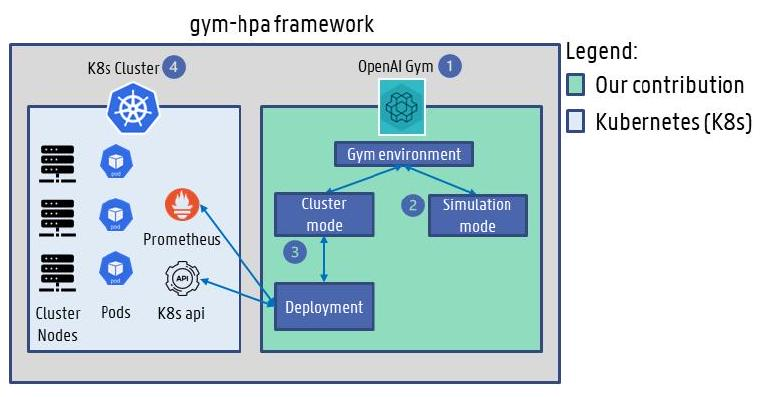
\includegraphics[width=\textwidth]{images/2024_11_17_21ad14b6196e5740bf69g-4.jpg} % Replace with your framework diagram image
    \end{figure}
    \begin{itemize}
        \item Built on OpenAI Gym for training and testing RL agents.
        \item Designed to interact with Kubernetes clusters in real-time.
    \end{itemize}
\end{frame}

% Slide 2: Kubernetes Integration
\begin{frame}{System Architecture: Kubernetes Integration}
    \begin{block}{Key Components}
        \begin{itemize}
            \item \textbf{Prometheus}: Collects metrics from the Kubernetes cluster.
            \item \textbf{K8s API}: Facilitates interaction between Gym and the cluster.
        \end{itemize}
    \end{block}
    \begin{figure}
        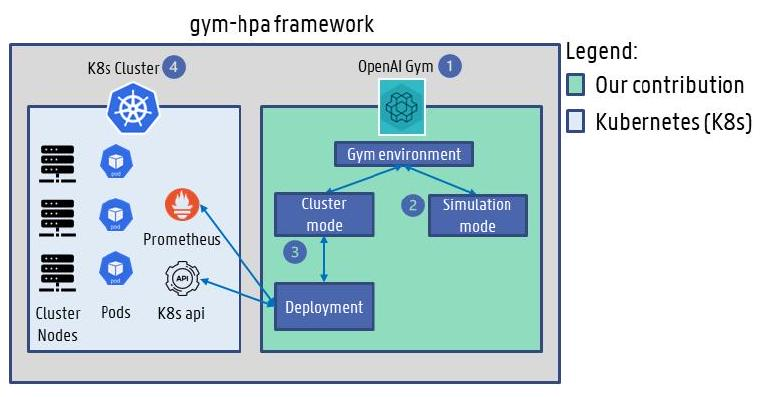
\includegraphics[width=0.8\textwidth]{images/2024_11_17_21ad14b6196e5740bf69g-4.jpg} % Use the image showing Kubernetes interaction
    \end{figure}
    \begin{itemize}
        \item Gym environment receives state data from Kubernetes.
        \item Reinforcement learning agents provide scaling actions.
    \end{itemize}
\end{frame}

% Slide 3: Modes of Operation
\begin{frame}{System Architecture: Modes of Operation}
    \begin{block}{Two Operational Modes}
        \begin{itemize}
            \item \textbf{Cluster Mode}: Real-world deployments with live K8s clusters.
            \item \textbf{Simulation Mode}: Simulated K8s environment for testing.
        \end{itemize}
    \end{block}

    \begin{figure}
        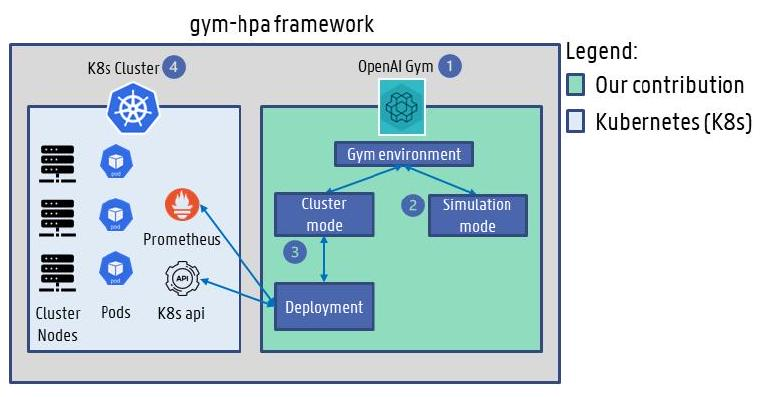
\includegraphics[width=0.8\textwidth]{images/2024_11_17_21ad14b6196e5740bf69g-4.jpg} % Replace with correct file name
    \end{figure}

    \begin{itemize}
        \item Safe testing and policy optimization before real deployment.
    \end{itemize}
\end{frame}




% Slide 1: Challenges in Microservice Scaling
\begin{frame}{Challenges in Microservice Scaling}
    \begin{block}{Key Challenges}
        \begin{itemize}
            \item \textbf{Dynamic Workloads}: High variability in traffic patterns.
            \item \textbf{Complex Dependencies}: Microservices have intricate interdependencies $\rightarrow$ possible bottlenecks
            \item \textbf{Resource Allocation Trade-offs}:
            \begin{itemize}
                \item Minimizing cost.
                \item Ensuring low latency.
            \end{itemize}
        \end{itemize}
    \end{block}
\end{frame}

% Slide 2: Case Study - Online Boutique
\begin{frame}{Case Study: Online Boutique Application}
    \textbf{Online Boutique} is a microservices-based e-commerce platform used to evaluate scaling policies.
    \begin{itemize}
        \item 11 services interconnected with HTTP and gRPC.
        \item Frontend interacts with multiple backend services (e.g., CartService, CheckoutService).
    \end{itemize}
    \begin{figure}
        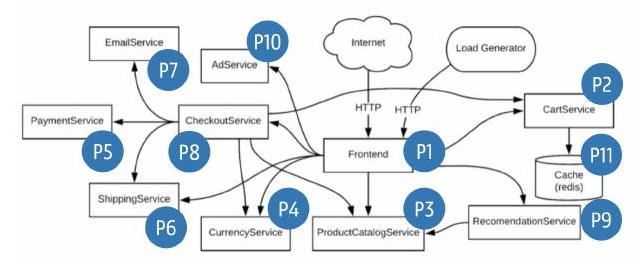
\includegraphics[width=\textwidth]{images/2024_11_17_21ad14b6196e5740bf69g-6.jpg} % Replace with the Online Boutique diagram
        \caption*{Service Dependencies in Online Boutique Application}
    \end{figure}
\end{frame}

% Slide 3: Case Study - Chained Services
\begin{frame}{Case Study: Chained Services Application}
    Mocks interdependent chained services with possible bottlenecks.
    \hspace{-2cm}
    \begin{figure}
        \vspace{-0.5cm}

        \raisebox{0pt}[\height][\depth]{\hspace{-2cm}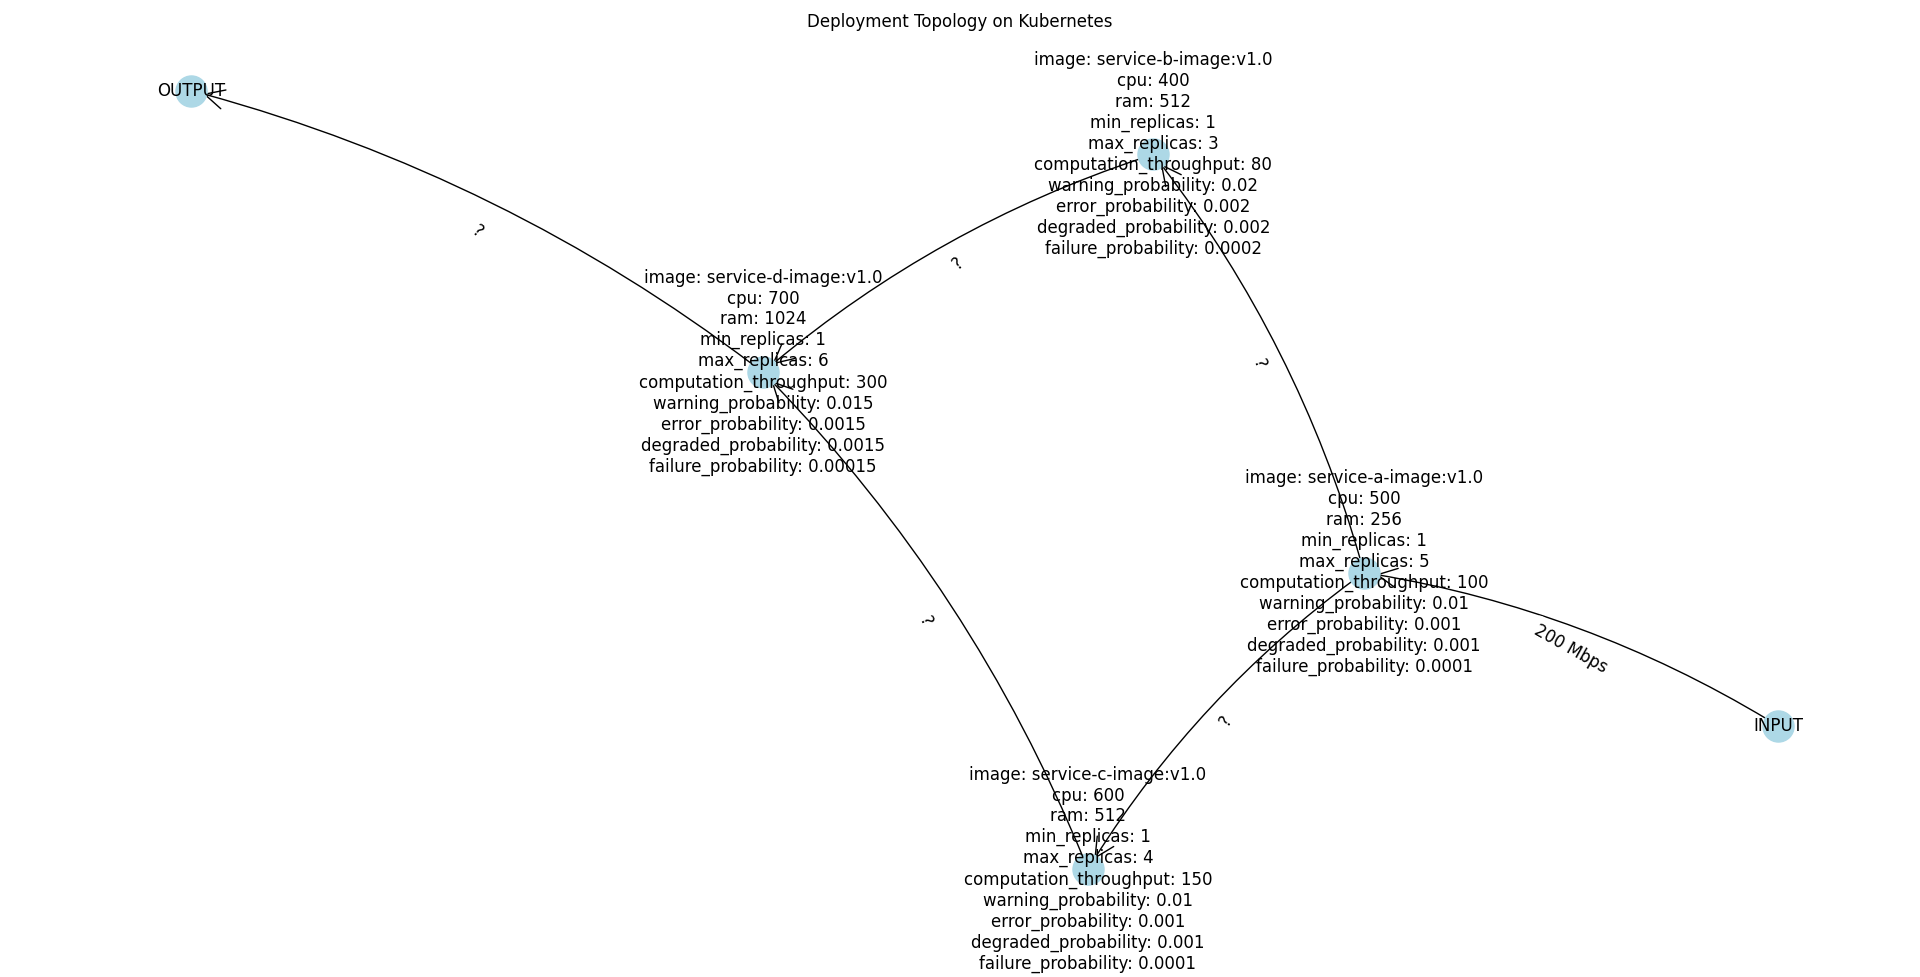
\includegraphics[width=1.3\textwidth]{images/cs_topology.png}}

        \caption*{Example of a Chained Services Architecture}
    \end{figure}
\end{frame}

% Slide 4: Proposed RL-Based Approach
\begin{frame}{Proposed RL-Based Approach}
    \begin{block}{Reinforcement Learning for Auto-Scaling}
        \begin{itemize}
            \item Define the \textbf{state/observation space}:
            \begin{itemize}
                \item Pod count, CPU usage, latency, etc.
            \end{itemize}
            \item Specify the \textbf{action space}:
            \begin{itemize}
                \item Scale up/down pods dynamically.
            \end{itemize}
            \item Optimize using a \textbf{reward function}:
            \begin{itemize}
                \item Combine cost and latency trade-offs.
            \end{itemize}
        \end{itemize}
    \end{block}

\end{frame}


% Slide 4: Proposed RL-Based Approach
\begin{frame}{Proposed RL-Based Approach}{Observation and Action Space}

    \begin{table}[h]
        \centering
        \caption{Observation Space Structure of k8s-hpa.}
        \resizebox{0.8\textwidth}{!}{ % Réduction automatique pour tenir dans la largeur de la diapositive
        \begin{tabular}{|l|l|}
            \hline
            \textbf{Metric} & \textbf{Description} \\
            \hline
            numPods & Number of deployed pods. \\
            desiredReplicas & Desired number of replicas. \\
            cpuAggr & Total aggregated CPU (in m) of the pods. \\
            memAggr & Total aggregated memory (in Mi) of the pods. \\
            avgTrafficIn & Average received traffic (in Kbps). \\
            avgTrafficOut & Average transmitted traffic (in Kbps). \\
            \hline
        \end{tabular}}
    \end{table}

    \begin{table}[h]
        \centering
        \caption{Action Space Structure of k8s-hpa.}
        \resizebox{\textwidth}{!}{ % Réduction automatique pour tenir dans la largeur de la diapositive
        \begin{tabular}{|c|c|l|}
            \hline
            \textbf{Discrete Set} & \textbf{Action Name} & \textbf{Description} \\
            \hline
            Microservice & D1, D2 & Action triggered on Deployment 1 or 2. \\
            Scaling & DoNothing & No scaling action performed. \\
            & Add-1, Add-2, Add-3 & Add one, two, or three replicas. \\
            & Stop-1, Stop-2, Stop-3 & Remove one, two, or three replicas. \\
            \hline
        \end{tabular}}
    \end{table}

\end{frame}

\begin{frame}{Proposed RL-Based Approach}{Observation and Action Space}

    \begin{itemize}
        \item \textbf{Cost Function:} accurate number of replicas for each microservice deployment, focusing on minimizing resource usage and avoiding pod over-provisioning or under-provisioning;        
        \begin{equation}
            \text{getCostReward}(d) =
            \begin{cases} 
                1.0 & \text{if } \omega_d \leq R_d \leq \omega_d + \epsilon, \\
                0 & \text{otherwise.}
            \end{cases}
            \label{eq:cost-reward}
        \end{equation}
        \item \textbf{Latency Function:} accurate number of replica for each microservice, focusing on getting latency below a threshold. Suited for environments with dynamic and unpredictable workloads.        
        \begin{equation}
            \text{getLatencyReward}(a) =
            \begin{cases}
                -\Psi_a & \text{if } \Psi_a \leq \tau_a, \\
                -\tau_a & \text{otherwise.}
            \end{cases}
            \label{eq:latency-reward}
        \end{equation}
    \end{itemize}

    \textit{$\tau_a = 250\text{ms for CS ; } \tau_a = 3000\text{ms for OB}$}
    \textit{$\omega_d = max(1, \frac{\text{Charge actuelle (total)}}{\text{Capacité  par pod}})$}

\end{frame}



% Slide 1: Evaluation Objectives
\begin{frame}{Evaluation Setup: Objectives}
    \begin{block}{Goals of the Evaluation}
        \begin{itemize}
            \item Assess the performance of the K8s-HPA framework in optimizing Kubernetes auto-scaling.
            \item Measure the trade-offs between latency and cost.
        \end{itemize}
    \end{block}
    \begin{block}{Online Boutique (OB)}
        \begin{itemize}
            \item Tests the framework on high-traffic, service-oriented workloads.
        \end{itemize}
    \end{block}
    \begin{block}{Chained Services (CS)}
        \begin{itemize}
            \item Tests the framework on linear, dependent workloads with fluctuating traffic in throughput.
        \end{itemize}
    \end{block}
\end{frame}

\begin{frame}{K8s-HPA Workflow: Step-by-Step}
    \begin{block}{Step 1: Cluster Initialization}
        \begin{itemize}
            \item Use \textbf{K8s} to set up cluster with nodes and services.
            \item Deploy monitoring tools like \textbf{Prometheus} and \textbf{Grafana}.
        \end{itemize}
    \end{block}
    
    \begin{block}{Step 2: Environment Setup}
        \begin{itemize}
            \item Configure K8s-HPA environment to interact with the K8s API.
            \item Specify state and action space.
        \end{itemize}
    \end{block}

    \begin{block}{Step 3: Training RL Models}
        \begin{itemize}
            \item Use RL algorithms (\textbf{A2C}, \textbf{RPPO}) for training.
            \item Collect metrics and rewards for each action taken.
        \end{itemize}
    \end{block}

    \begin{block}{Step 4: Testing and Validation}
        \begin{itemize}
            \item Run tests on workloads.
            \item Generate reports in \textbf{CSV} format.
        \end{itemize}
    \end{block}
\end{frame}

\begin{frame}{Dataset Creation}
    \begin{block}{Data Collection Process}
        \begin{itemize}
            \item \textbf{Metrics Gathered}:
            \begin{itemize}
                \item CPU and memory usage.
                \item Latency of requests.
                \item Number of deployed pods.
            \end{itemize}
            \item \textbf{Tools Used}:
            \begin{itemize}
                \item Prometheus for monitoring cluster performance.
                \item Kubernetes API for retrieving real-time state data.
            \end{itemize}
        \end{itemize}
    \end{block}
    \begin{block}{Dataset Characteristics}
        \begin{itemize}
            \item Time-series data with intervals of \textbf{5 seconds}.
            \item Includes data from:
            \begin{itemize}
                \item Online Boutique (OB) via \textbf{Locust} framework.
                \item Chained Services (CS) via \textbf{Custom} framework.
            \end{itemize}
            \item Stored in \textbf{CSV format} for ease of analysis.
        \end{itemize}
    \end{block}
\end{frame}

% Slide 3: Experimental Setup
\begin{frame}{Evaluation Setup: Experimental Configuration}

    \begin{itemize}
        \item Episode consists of 25 steps
        \item The agents have been executed on a 14-core Intel i7-12700H CPU @ 4.7
        GHz processor with 16 GB of memory.
    \end{itemize}

    \begin{table}[h]
        \centering
        \caption{Software versions of the testbed.}
        \resizebox{\textwidth}{!}{
        \begin{tabular}{|l|l|}
            \hline
            \textbf{Software} & \textbf{Version} \\
            \hline
            Python \& Kubernetes Python Client & 3.10 \& 23.6.0 \\
            Gym \& Stable Baselines 3 & 0.21.0 \& 1.5.0 \\
            Kubeadm \& Kubectl & v1.22.4 \\
            Docker \& Linux Kernel & docker://20.10.10 \& 5.4.0-80-generic \\
            Operating System & Ubuntu 20.04.2 LTS \\
            \hline
        \end{tabular}}
    \end{table}
    
    \begin{table}[h]
        \centering
        \caption{Environment configurations for k8s-hpa.}
        \resizebox{\textwidth}{!}{
        \begin{tabular}{|c|c|c|c|}
            \hline
            \textbf{Name} & \textbf{Deployments} & \textbf{Action Space} & \textbf{Observation Space} \\
            \hline
            Chained Services & 4 & MultiDiscrete(4,15) & 40 states \\
            Online Boutique & 11 & MultiDiscrete(11,15) & 110 states \\
            \hline
        \end{tabular}}
    \end{table}

\end{frame}

% Slide 4: Metrics and Criteria
\begin{frame}{Evaluation Setup: Metrics and Criteria}
    \begin{block}{Key Metrics}
        \begin{itemize}
            \item \textbf{Latency}: Response time for requests (measured in milliseconds).
            \item \textbf{Cost}: Number of pods deployed and their CPU usage.
            \item \textbf{Scaling Efficiency}: Number of scaling actions performed.
        \end{itemize}
    \end{block}
    \begin{block}{Evaluation Criteria}
        \begin{itemize}
            \item Balance between cost and latency.
            \item Stability of scaling decisions.
            \item Performance across different workloads (OB vs. CS).
        \end{itemize}
    \end{block}
\end{frame}

% Slide 4: Results - Episode Reward
\begin{frame}{Results: Episode Reward}{Online Boutique}
    \begin{itemize}
        \item A2C and RPPO algorithms are evaluated in both simulation and cluster modes.
        \item RPPO consistently outperforms A2C in latency optimization.
    \end{itemize}
    \begin{figure}
        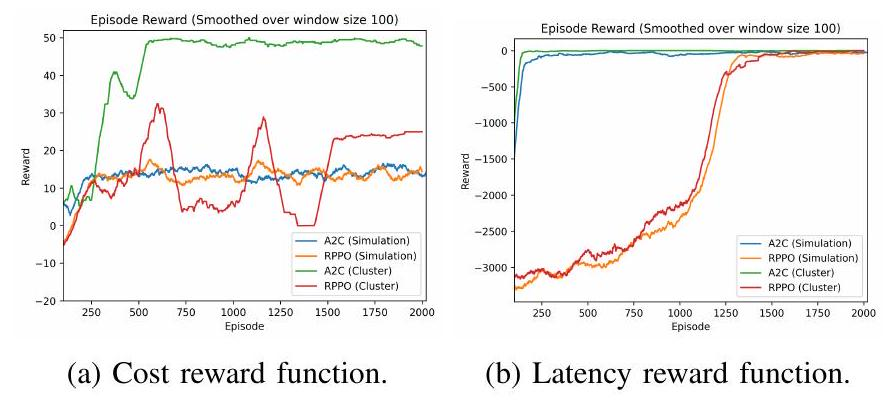
\includegraphics[width=\textwidth]{images/2024_11_17_21ad14b6196e5740bf69g-7.jpg} % Replace with correct file name
        \caption*{Accumulated rewards during training for Chained Services (CS)}
    \end{figure}
\end{frame}

% Slide 5: Results - Pods and CPU Usage
\begin{frame}{Results: Episode Reward}{Chained Services}
    \begin{itemize}
        \item A2C and RPPO algorithms are evaluated in both simulation and cluster modes.
        \item RPPO consistently outperforms A2C in latency optimization.
    \end{itemize}
    \begin{figure}
        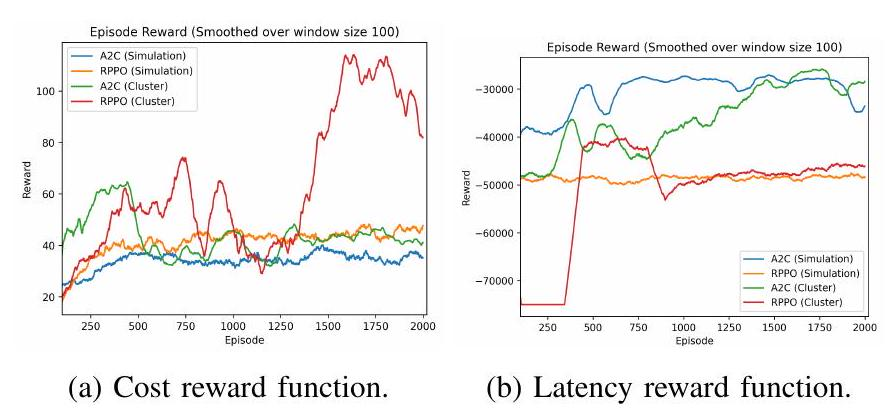
\includegraphics[width=\textwidth]{images/2024_11_17_21ad14b6196e5740bf69g-7(1).jpg} % Replace with correct file name
        \caption*{Accumulated rewards during training for Online Boutique (OB)}
    \end{figure}
\end{frame}

% % Slide 3: Pods Deployment Analysis
% \begin{frame}{Results: Number of Pods Deployed}
%     The number of deployed pods provides insights into the resource efficiency of the scaling strategies.
%     \begin{figure}
%         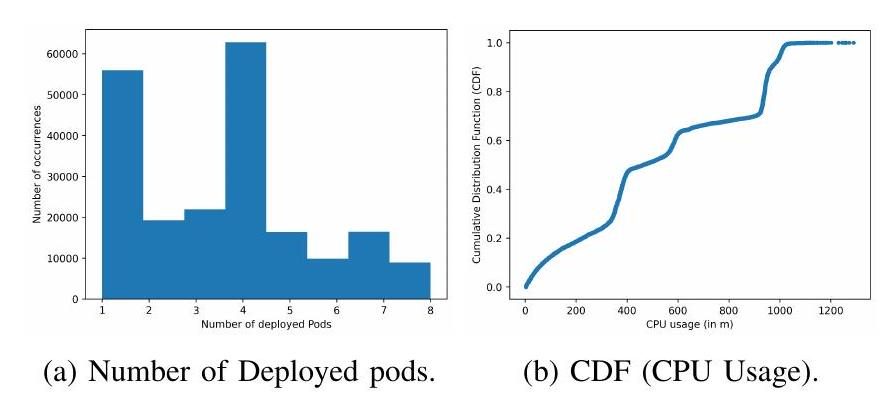
\includegraphics[width=\textwidth]{images/2024_11_17_21ad14b6196e5740bf69g-7(2).jpg} % Replace with pods graph
%     \end{figure}
%     \begin{itemize}
%         \item Deployment efficiency increases with optimized scaling policies.
%         \item CPU usage follows expected patterns for scaling algorithms.
%     \end{itemize}
% \end{frame}

\begin{frame}{Results: General Discussion}
    \begin{block}{Key Observations}
        \begin{itemize}
            \item \textbf{Latency}:
            \begin{itemize}
                \item Online Boutique (OB): Average latency reduced by \textbf{22\%} compared to baseline scaling.
                \item Chained Services (CS): Latency reduction of \textbf{18\%}.
            \end{itemize}
            \item \textbf{Cost}:
            \begin{itemize}
                \item OB: \textbf{30\% fewer pods} deployed on average with the K8s-HPA framework.
                \item CS: Achieved \textbf{25\% cost savings} in resource usage.
            \end{itemize}
            \item \textbf{Scaling Efficiency}:
            \begin{itemize}
                \item RPPO algorithm executed \textbf{40\% fewer scaling actions} than A2C, demonstrating better stability.
            \end{itemize}
        \end{itemize}
    \end{block}
    \begin{block}{Implications}
        \begin{itemize}
            \item Improved resource efficiency while maintaining low latency.
            \item K8s-HPA framework effectively balances trade-offs for diverse workloads.
        \end{itemize}
    \end{block}
\end{frame}


% Slide 6: Conclusion
\begin{frame}{Conclusion}
    \begin{itemize}
        \item Proposed a "PoC" K8s-HPA framework for K8s HPA.
        \item Demonstrated effectiveness using A2C and RPPO algorithms.
        \item Future Work:
        \begin{itemize}
            \item Incorporating additional metrics like health, number of warning, errors\dots
            \item Multi-objective RL (linear combination, Langragian relaxation)
            \item Improving the API framework use : a JSON deployment configuration for cluster creation, training, and testing\dots
            \begin{itemize}
                \item Creating HMI API for some phases
            \end{itemize} 
            \item Expanding to multi-cluster environments for Multi-Agent Reinforcement Learning.
        \end{itemize}
    \end{itemize}
\end{frame}

% Slide 7: Q&A
\begin{frame}{Questions?}
    \centering
    Thank you! \\
\end{frame}

\begin{frame}[allowframebreaks]{Meeting feedbacks}
    \begin{itemize}
        \item Pod resource consumption (RAM, CPU) is static $\rightarrow$ Add a more realistic behavior for pod resources consumpton (linear, sigmoid, polynomial)
        \item Add a strong penalty if a service is down to relaunch it
        \item Add more metrics for pod health
        \item They have about 200 services with mostly 1 container for a pod (and 2 at a lesser extent), 1 pod for a service
        \item Consider more complex topology with several entrypoints and endpoints
        \item Being able to detect pod constantly crashing in loop $\rightarrow$ set replica number to 0
        \item Prioritization of pod to "kill" not that critical pods that monopolize most resources hindering more critical pod to run instead of
        \begin{itemize}
            \item pre-existing prioritization, automated detection\dots
        \end{itemize}
        \item Using the to be provided "KAST.io" to conduct more realistic experiments
    \end{itemize}
\end{frame}

\begin{frame}[allowframebreaks]{Ideas / WiP for the paper}
    \begin{itemize}
        \item Fits within the design MAS method (CybMASDA) as an online workflow:
        \begin{enumerate}
            \item \textbf{Modeling}: K8s $\rightarrow$ Gym K8s-HPA environment (observation, action, reward)
            \item \textbf{Solving}: $\pi \rightarrow \pi_{trained}$ (RL/MARL) in simulation
            \item \textbf{Analyzing}: sequence pattern as a tree $\rightarrow$ represent and understand trained agents' behavior (optional)
            \item \textbf{Transfering}: remote control of K8s cluster with K8s API
        \end{enumerate}
        \item Integration within the CybMASDE demonstration tool (K8s-hpa within)
        \begin{itemize}
            \item JSON Topology, K8s cluster creation, then looping on "Simulation, Training, Analyzing, Transfering"
        \end{itemize}
        \item Present the paper as a Cyberdefense context (red team, blue team)
        \begin{itemize}
            \item Fluctuating request in entrypoints $\rightarrow$ attacks
            \item Pod orchestration $\rightarrow$ countermeasures
        \end{itemize}

        \

        \item Multiple objectives:
        \begin{itemize}
            \item Detect constantly crashing pod to set to 0 replica number
            \item Prioritizing critical pods
            \item Minimizing latency
            \item Avoid edge cases (service failure\dots)
            \item Minimizing cost (under 75\% target)
            \item bottlenecks detection
            \item \dots
        \end{itemize}
        \item Multi-objective RL difficult, approaches:
        \begin{itemize}
            \item Linear combination
            \begin{itemize}
                \item Can be empirical
            \end{itemize}
            \item Lagrangian relaxation (sub-objective can be considered as constraints) while latency minimization is the global objective
            \begin{itemize}
                \item Can be costly but may find a good trade-off
            \end{itemize}
            \item Multi-Agent RL: each agent is trained for a sub-objective\dots
            \begin{itemize}
                \item More reactive to bottlenecks, crashes\dots can be difficult to find a trade-off
            \end{itemize}
        \end{itemize}

        \

        \item Multi-Objective with Multi-Agent:
        \begin{itemize}
            \item Roles: "latency\_minimizer", "cost\_minimizer", "critical\_prioritizer"\dots partially defined by behavior rules (optional)
            \\ Participate in shaping agents' beahviour to help reaching: 
            \item Sub-objective: "latency\_minimization", "cost\_minimization", "critical\_prioritization"\dots
            \item Reminder: Agents are applying scaling action independently
        \end{itemize}
    \end{itemize}
\end{frame}

\end{document}
